% Generated by Scripts/build-release-documents.py from release Markdown.
\documentclass[11pt,letterpaper]{article}
\usepackage[margin=1in]{geometry}
\usepackage[T1]{fontenc}
\usepackage{tgpagella}
\pdfinterwordspaceon
\usepackage{enumitem}
\setlist[itemize]{leftmargin=*,itemsep=.1em}
\usepackage{pdfpages}
\usepackage[colorlinks=true,urlcolor=blue,linkcolor=blue]{hyperref}
\hypersetup{pdftitle={TeXShop Changes},pdfauthor={TeXShop contributors}}
\setcounter{secnumdepth}{0}
\setlength{\parindent}{0pt}
\setlength{\parskip}{.3em}
\setlength{\emergencystretch}{2em}
\begin{document}
\section{TeXShop 5.60}

\noindent\textit{Release preparation; not yet published.}\par

TeXShop 5.60 fixes typesetting cancellation and improves LaTeX-aware spell checking, external file monitoring, editing long documents, and Settings.


\subsection{Typesetting and stability}

\begin{itemize}
\item \textbf{Critical fix:} Fix a problem where Stop reported that typesetting had been aborted but left TeX running. Starting another typesetting job now also stops the previous job and its child processes.
\item Handle failures to launch typesetting tools and missing command-search paths more reliably, and avoid an indefinite wait when stopping helper processes.
\item Show a sheet when a specified TeX root file cannot be found.
\item Fix errors involving empty documents, isolated quotation marks, and save-completion handling.
\item Improve the handling of console output and log files that contain mixed encodings or broken characters. Read affected output line by line, trying UTF-8 and then the document’s encoding, with Latin 9 as a last resort. Keep unreadable data from spoiling other lines, and rejoin UTF-8 characters split by TeX’s line wrapping.
\end{itemize}

\subsection{LaTeX-aware spell checking}

\begin{itemize}
\item Add LaTeX-aware spell checking, based on suggestions from Ralph Martin. It checks prose while skipping TeX commands, comments, mathematics, and arguments used for references and similar purposes. The feature is enabled by default and can be turned off under Settings \(\rightarrow\) Source.
\item Recognize supported macro definitions and language-switching commands when identifying text to check. The spelling panel can check passages in the specified language.
\item Add editable spelling-exclusion rules, a replacement field and Change All for words in the checked text, and a way to forget learned words found in the current document. A Change All operation can be undone in one step.
\item Fill the replacement field for Change All with the suggestion selected in the spelling panel, by clicking it or with the arrow keys. When there is only one suggestion, it is filled in as soon as the word is shown. The text changes only when Change All is used.
\item Improve Find Next, scrolling to misspelled words, and spell-checking performance in long documents and split editors.
\end{itemize}

\subsection{External file changes and PDF preview}

\begin{itemize}
\item Make source-file monitoring continue after automatic reloads and file replacement by external editors, including atomic saves. Preserve unsaved edits and the undo history for TeXShop’s own saves. This includes the contribution from ddd3h in PR \#1.
\item When Automatic Preview Update is enabled, detect PDFs changed by other applications and reload the preview while preserving the page position and zoom. Avoid replacing unsaved PDF annotations, and retry when an external writer temporarily leaves an incomplete PDF.
\item Move file-change checks off the main thread to keep the interface responsive.
\item Fix a PDFKit crash during preview reloads, including changes in page count, by correcting how PDF documents are shared with the second preview pane.
\item Correct Space and Shift-Space scrolling when a PDF page is larger than the preview window.
\item Add Page Layout and Two-Page Arrangement menus to the preview toolbar. Page Layout changes the page layout of the current document. Two-Page Arrangement changes the page direction and whether the first page is shown alone as a cover; Restore Document Settings returns these two to the document’s settings. The changes last until the document is closed. The page being viewed and the zoom are kept when the layout or arrangement changes.
\item Add a check box under Settings \(\rightarrow\) Preview, formerly a hidden setting, to show the first page alone as a cover in two-page layouts. Use the page direction recorded in the PDF unless a magic comment specifies the direction. These settings apply to documents opened afterward, and magic comments take precedence over them.
\end{itemize}

\subsection{Editing and keyboard navigation}

\begin{itemize}
\item Edit menu shortcuts in Settings \(\rightarrow\) Keyboard. Search by Function finds command names; Search by Key records a key to show matching menu commands and macros, including inactive assignments. Show in Macro Editor selects the matching macro without discarding unsaved edits. Commands can be searched, a new shortcut is recorded by pressing it, shortcuts already in use are reported, and one or all shortcuts can be restored. Changes take effect immediately and are kept after restarting. Shortcuts set in KeyEquivalents.plist remain the defaults. Menu commands take precedence over macros; macros can use keys freed by customization. Confirm before assigning a macro’s key to a menu command. The Macro Editor marks inactive shortcuts, identifies the conflicting command and key, and asks about new or changed conflicts when saving; existing unchanged conflicts do not interrupt saving. The bundled New array macro now uses Control-Shift-Command-A.
\item Improve opening, scrolling, and editing long source documents by laying out text where needed and reducing repeated paragraph-layout work. Limit matching-brace searches on cursor movement.
\item Preserve explicit left alignment in right-to-left paragraphs.
\item Use Command-0 to show the current document’s console. Press it again in the console to return to the source or PDF window that opened it; if there is no originating window, return to the source. This follows the existing Command-1 behavior.
\item Keep the Tags menu correctly localized when reopening a document in the combined source-and-preview window.
\end{itemize}

\subsection{Opening and saving documents}

\begin{itemize}
\item Detect the encoding of a file that has no encoding magic comment when it is opened. Unicode files with or without a byte order mark, Japanese, Chinese and Korean files, and files in one-byte encodings of the user’s languages are recognized, with the encoding declared to inputenc as a hint. A hidden setting turns the detection off.
\item Keep the byte order mark of UTF-8 files and the byte order of UTF-16 files when saving, and read encoding magic comments in UTF-16 files.
\item Read GB 2312 files correctly, and stop a file that could not be read in its specified encoding from being damaged when it is saved.
\item Always write TeX’s backslash and tilde as the bytes 0x5C and 0x7E in Japanese encodings. A typed backslash or tilde no longer becomes a full-width backslash or wave dash, or the byte 0x80, in Mac Japanese and Shift JIS X0213 files, and a yen sign typed for a backslash no longer becomes “?” in Windows Shift JIS, EUC-JP and ISO-2022-JP files.
\item Use UTF-8 rather than Latin 9, with a message, when an encoding name is not recognized, and write project files in UTF-8.
\item When an opened file has Windows (CRLF), classic Mac (CR) or mixed line endings, tell the user that they have been changed to LF. The notice can be turned off for each file.
\item Fix the encoding menu in the Save dialog, which did not change the encoding of the saved file. The menu can now be shown from Settings \(\rightarrow\) Misc1. When the source has an encoding magic comment naming a known encoding, the menu shows that encoding and cannot be changed, unless the file could not be read in that encoding.
\item Add settings under Settings \(\rightarrow\) Misc1 to turn autosave and Versions on or off and, while autosave is off, to keep the previous file as “name\textasciitilde{}” when saving.
\end{itemize}

\subsection{App and Dock icons}

\begin{itemize}
\item Introduce a white-frame app icon inspired by the classic circular icon, with optically centered TeX lettering and a rounded-square shape for current macOS versions.
\item Add five Dock icon choices under Settings \(\rightarrow\) Misc2, including historical designs. The selected icon retains its original shape while TeXShop is running, without a separate background process. After quitting, the Dock returns to the standard app icon; the Finder icon is unchanged.
\end{itemize}

\subsection{Settings and themes}

\begin{itemize}
\item Find TeX and Ghostscript installations automatically. When TeXShop is first used, and with Auto Setup… under Settings \(\rightarrow\) Engine, the installations found are listed with their versions. The newest is selected, and another can be chosen for TeX and for Ghostscript separately. The paths change only after confirmation; custom engines and the alternate path are not changed.
\item Correct overlapping controls, clipped labels, and incorrect control connections throughout the localized Settings windows. Add missing bracket-color controls in Dutch.
\item Choose the markers for spaces, full-width spaces, newlines and tabs from pop-up menus under Settings \(\rightarrow\) Editor, with more choices for newlines and tabs.
\item Show bracket and expl3 colors from the theme being edited, update inherited colors correctly, and preserve the theme when a color change is ignored. Older themes without bracket colors use the marker color.
\item Use a resizable Settings window with a category sidebar and Back/Forward navigation. Command-left bracket and Command-right bracket navigate Settings while that window is active, taking precedence over menu shortcuts there. The last category is remembered; navigation history is cleared when Settings closes. Store settings under the application’s bundle identifier. Save valid Settings changes as they are made; close the window with the close button or Command-W. Text fields are checked on Return, focus changes, navigation, and closing. Invalid entries keep their last saved value; there is no whole-window OK or Cancel. Auto Save changes are saved immediately but take effect after restarting TeXShop.
\item Save theme edits immediately and update documents only after the theme file has been written successfully. Duplicate a theme before editing to keep the original. A failed save restores the last saved colors; selecting a theme to edit does not temporarily apply it to every document.
\item Save the selected Dock icon immediately. Closing Settings keeps the choice; applying a settings profile restores the current app icon.
\item Use the zoom setting as the default for newly opened PDFs, preserving the zoom of existing PDFs. Source and console font changes still update open windows immediately.
\item Apply settings profiles after showing their reset scope and TeX engine path. Reset known editing, engine, display, hidden settings, and the running Dock icon; preserve shortcuts, system language, window layouts, automatic updates, theme files, and unrecognized settings. Theme selections may change.
\item Fix Make Default Editor for .tex files.
\item Add an option under Settings \(\rightarrow\) Editor to treat @ as part of command names in syntax coloring.
\item Add an option under Settings \(\rightarrow\) Editor to color expl3 code by default. Each document reads it when it opens, and the Source menu still turns expl3 coloring on or off for a single document.
\item Standardize the Settings terminology, remove obsolete PDFSync choices and ineffective settings, and consistently use the modern toolbar icons.
\end{itemize}

\subsection{Help and source distribution}

\begin{itemize}
\item Add help for LaTeX-aware spell checking, repair broken help links, and update the hidden-settings reference.
\item Fix a resource filename that could prevent building TeXShop from an extracted source archive.
\end{itemize}

\subsection{Bundled libraries}

\begin{itemize}
\item Update the bundled zlib to 1.4 and the SyncTeX parser to 1.21.
\end{itemize}
\clearpage
\section{TeXShop 5.59}

This is the first TeXShop release maintained by Yusuke Terada, following Richard Koch's handover of the project. It builds on TeXShop 5.58 Golden Gate.


\subsection{Changes}

\begin{itemize}
\item Keep the PDF zoom indicator in sync with trackpad gestures and preserve manual zoom when reloading a PDF.
\item Correct initial PDF positioning and preview overlay coordinates.
\item Add a PDF appearance menu with System, Light, and Dark choices.
\item Fix toolbar item sizing and localized Preferences layouts and fonts.
\item Create HTML preview views at runtime to avoid document-window loading failures on older macOS versions.
\item Enable macOS filename suggestions for untitled documents on macOS 27.
\item Fix a syntax-highlighting range error that could cause a crash.
\item Align invisible-character markers with the text baseline.
\item Restore the preview after a failed compilation produces an invalid PDF and a subsequent compilation succeeds.
\item Work around a PDFKit/Metal rendering crash on macOS 27.
\item Introduce a new app icon and update Sparkle to 2.10.1, using the update feed at texshop.app.
\item Make the Spotlight importer native on Apple Silicon while retaining Intel support.
\item Update About credits to identify the current maintainer and original developer.
\end{itemize}

\subsection{Installation}

Download \texttt{TeXShop-5.59.zip}, extract it, and copy TeXShop.app to Applications. A separate TeX distribution, such as MacTeX, is required for typesetting.


Official website: \url{https://texshop.app/}


The application is built for Apple Silicon and Intel with a minimum deployment target of macOS 14.6.


Users of Richard Koch's earlier releases should install this release manually. This release uses a new update feed for subsequent TeXShopProject updates.

\clearpage
\pdfbookmark[0]{TeXShop 5.57 and earlier}{historical-changes}
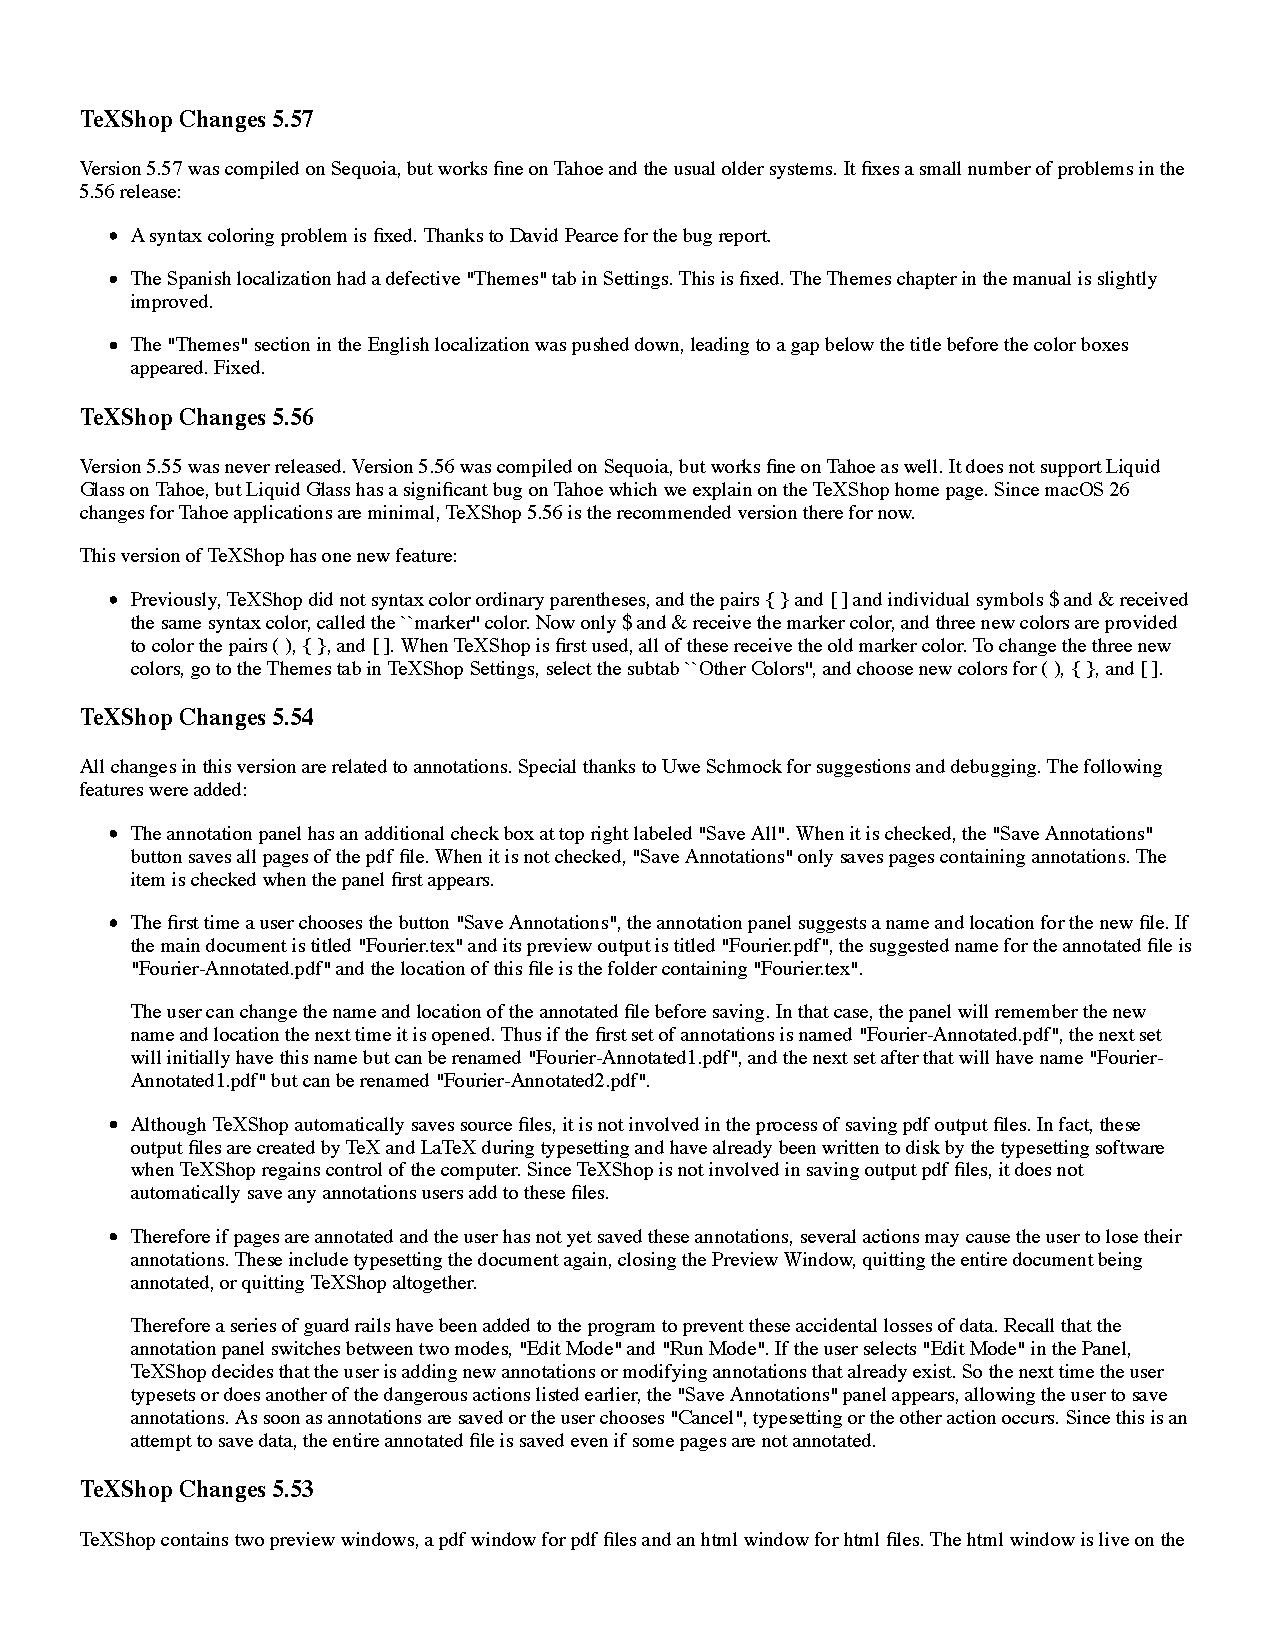
\includepdf[pages=-]{Changes-5.57.pdf}
\end{document}
